\documentclass{standalone}

\usepackage{tikz}
\usetikzlibrary{calc}

\begin{document}

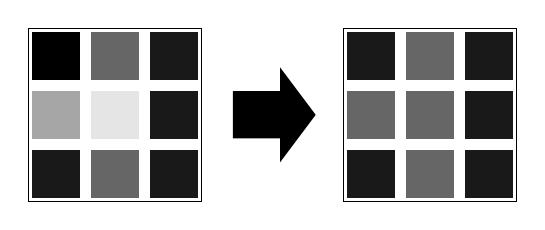
\begin{tikzpicture}
   \def\sqwi{0.6}
   \def\sqwi{0.6}
   \def\sechs{black!100!white}
   \def\funf{black!90!white}
   \def\vier{black!60!white}
   \def\zwei{black!35!white}
   \def\eins{black!10!white}
   \def\null{black!0!white}
   \begin{scope}[local bounding box = scope1] 
       \draw (-0.65,-0.05) rectangle (1.55,2.15);
       \draw[color=\funf, fill] (0,0) rectangle node{5} (0-\sqwi,0+\sqwi);
       \draw[color=\vier, fill] (0.75,0) rectangle node{4} (0.75-\sqwi,0+\sqwi);
       \draw[color=\funf, fill] (1.5,0) rectangle node{5} (1.5-\sqwi,0+\sqwi);
       \draw[color=\zwei, fill] (0,0.75) rectangle node{2} (0-\sqwi,0.75+\sqwi);
       \draw[color=\eins, fill] (0.75,0.75) rectangle node{1} (0.75-\sqwi,0.75+\sqwi);
       \draw[color=\funf, fill] (1.5,0.75) rectangle node{5} (1.5-\sqwi,0.75+\sqwi);
       \draw[color=\sechs,fill] (0,1.5) rectangle node{6} (0-\sqwi,1.5+\sqwi);
       \draw[color=\vier, fill] (0.75,1.5) rectangle node{4} (0.75-\sqwi,1.5+\sqwi);
       \draw[color=\funf, fill] (1.5,1.5) rectangle node{5} (1.5-\sqwi,1.5+\sqwi);
    \end{scope}
    \begin{scope}[xshift = 5.5cm, yshift=4.5cm, transform canvas={scale=0.3}]
       \fill[color=black] (1,0) --(3,0) --(3,1) --(4.5,-1) -- (3,-3) -- (3, -2) -- (1,-2);
    \end{scope}
    \begin{scope}[xshift = 4cm]
        \draw (-0.65,-0.05) rectangle (1.55,2.15);
        \draw[color=\funf, fill] (0,0) rectangle node{5} (0-\sqwi,0+\sqwi);
        \draw[color=\vier, fill] (0.75,0) rectangle node{4} (0.75-\sqwi,0+\sqwi);
        \draw[color=\funf, fill] (1.5,0) rectangle node{5} (1.5-\sqwi,0+\sqwi);
        \draw[color=\vier, fill] (0,0.75) rectangle node{4} (0-\sqwi,0.75+\sqwi);
        \draw[color=\vier, fill] (0.75,0.75) rectangle node{4} (0.75-\sqwi,0.75+\sqwi);
        \draw[color=\funf, fill] (1.5,0.75) rectangle node{5} (1.5-\sqwi,0.75+\sqwi);
        \draw[color=\funf, fill] (0,1.5) rectangle node{5} (0-\sqwi,1.5+\sqwi);
        \draw[color=\vier, fill] (0.75,1.5) rectangle node{4} (0.75-\sqwi,1.5+\sqwi);
        \draw[color=\funf, fill] (1.5,1.5) rectangle node{5} (1.5-\sqwi,1.5+\sqwi);
    \end{scope}
\end{tikzpicture}

\end{document}
